%\documentclass[manuscript]{aastex} %one-column, double-spaced document
%%\documentclass[preprint2]{aastex} %double-column, single-spaced document:
%\documentclass[preprint]{aastex}
\documentclass[iop,floatfix]{emulateapj}
\usepackage{apjfonts}
\usepackage{hyperref}

\shorttitle{HW 1: MCMC}

\begin{document}
\title{HW 1 Solutions: Fitting a straight line with MCMC}
\author{}
\affil{Harvard University\\
  Department of Astronomy\\
  60 Garden Street MS 10\\
Cambridge, MA 02138}

\begin{abstract}
We use a Metropolis-Hastings Markov Chain Monte Carlo (MCMC) method to determine the best-fit parameters for a straight line to noisy data.
\end{abstract}

\section{Data and parameter estimates}
Before writing any code\footnote{All code used for analysis and plotting is available at \url{https://github.com/iancze/AY193/tree/master/HW1}} to fit the data, you should first plot the data to get an idea of what parameter space you are dealing with. Estimates of the parameters are made as shown in Figure~\ref{fig:basic_plot} and listed in Table~\ref{table:part_a}. We are also told from the handout that $\sigma_i = \sigma = 0.1$. The estimates of $a$ and $b$ ($a_e$ and $b_e$) are made by simply playing around with a ruler on a printout of the data, varying the parameters until we arrive at what looks like a best fit. The estimate in $\sigma$ ($\sigma_e$) is made by assuming the best fit line and then characterizing the typical scatter about this line. Estimates of $\sigma_a$ and $\sigma_b$ ($\sigma_{a,e}$ and $\sigma_{b,e}$) are made by keeping $b$ fixed while varying $a$ (or vice-versa) in order to determine the range of $a$ (or $b$) values which would still give an acceptable fit to the data. 

\begin{figure}
\begin{center}
  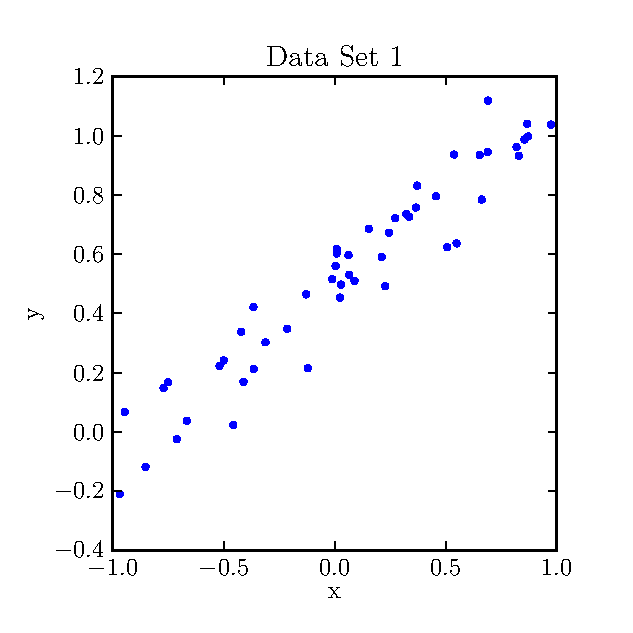
\includegraphics[width=0.5\textwidth]{basic_plot}
  \caption{Parameter estimates done by eye. $\sigma$ can be estimated from the scatter about the best fit line, done by eye. $\sigma_a$ and $\sigma_b$ can be estimated by varying $a$ or $b$ while keeping the other fixed, and finding the range of values for which the line still fits. Parameter estimates are shown in Table~\ref{table:part_a}.}
\label{fig:basic_plot}
\end{center}
\end{figure}

\begin{deluxetable}{ll}
\tablecaption{\label{table:part_a} Parameter Estimates}
\tablehead{\colhead{Parameter} & \colhead{Value}}
\startdata
$a_e$ & 0.5 \\
$b_e$ & 0.6 \\
$\sigma_e$ & 0.1 \\
$\sigma_{a,e}$ & 0.03 \\
$\sigma_{b,e}$ & 0.05 \\
\enddata
\tablecomments{Your own values may vary slightly, after all, they are estimates by eye.}
\end{deluxetable}

\section{The Likelihood of the Model}

As detailed in the handout, let $x_i$ and $y_i$ be our data, and the line model described as 
\begin{equation}
  f(p_n,x_i) = a + b x_i
\end{equation}
where $p_n = \{a,b\}$.

We characterize the goodness of fit by the $\chi^2$ statistic
\begin{equation}
  \chi^2 = \sum_{i=1}^N \left [\frac{y_i - f(p_n,x_i)}{\sigma_i} \right ]^2
  \label{eqn:chi_sq}
\end{equation}

where in this problem we have assumed $\sigma_i = \sigma$. The ``likelihood'' of having a particular data set generated by the parameters is 
\begin{equation}
  {\cal L} = \exp(-\chi^2/2)
  \label{eqn:likelihood}
\end{equation}

Calculating ${\cal L}$ for a given $p_n$ is likely to be computationally intensive, since Eqn~\ref{eqn:chi_sq} involves squaring and summing operations for $N$ data points. If we have a simple model and a moderate number of data points, it is sometimes quickest to just sample ${\cal L}$ over a grid of $p_n$, and by visual inspection find the maximum. We can of course use any other gradient optimization techniques to find the maximum. Even if the model is complicated, it might be worth it to sample the parameter space with a coarse grid, simply to get an idea of what you are dealing with beforehand. The ${\cal L}$ space of our problem is shown in Figure~\ref{fig:likelihood}. This is the probability space which our Markov chain will sampling.

\begin{figure}
\begin{center}
  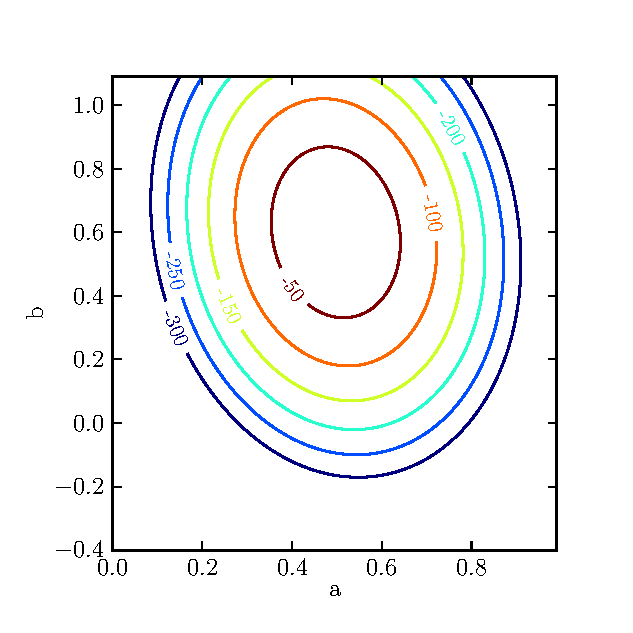
\includegraphics{likelihood}
  \caption{The ${\cal L}$ space sampled on a grid. Contours show $\log_{10}({\cal L})$, and so many of the values are negative. Note how strongly peaked the probability distribution is around $a=0.5$,$b=0.6$. This likelihood space will be sampled by our Markov Chain Monte Carlo algorithm.}
\label{fig:likelihood}
\end{center}
\end{figure}

\section{The MCMC Algorithm}

We sample the likelihood space (Figure~\ref{fig:likelihood}) with the Markov Chain Monte Carlo (MCMC) algorithm. First, we assume some starting combination of parameters, $p_{\rm start} = \{a_{\rm start}, b_{\rm start}\}$.

In each iteration of the algorithm, we jump in the likelihood space 

\begin{eqnarray}
  a_j &= a_{j-1} + \Delta a_j \\
  b_j &= b_{j-1} + \Delta b_j
\end{eqnarray}

where $\Delta a_j$ and $\Delta b_j$ are drawn from Gaussian distributions

\begin{eqnarray}
  \Delta a_j &\propto P_G(\mu = 0, \sigma = \sigma_{\Delta a})\\
  \Delta b_j &\propto P_G(\mu = 0, \sigma = \sigma_{\Delta b})
\end{eqnarray}

where $P_G$ is a generic Gaussian distribution with mean $\mu$ and standard deviation $\sigma$. You may use a Gaussian random number generator within your code. For example, one \verb|Python| routine is \verb|np.random.normal|. We use our estimates in Table~\ref{table:part_a} for $\sigma_{a,e}$ and $\sigma_{b,e}$ to set the jump distribution width ($\sigma_{\Delta a}$ and $\sigma_{\Delta b}$) accordingly

\begin{eqnarray}
  \sigma_{\Delta a} &\approx \sigma_{a,e}\\
  \sigma_{\Delta b} &\approx \sigma_{b,e}\\
\end{eqnarray}

Later on in the problem set, we will vary $\sigma_{\Delta a}$ and $\sigma_{\Delta b}$ to asses their impact on the efficiency of the MCMC algorithm. After taking a jump (moving from $j -1 $ to $j$), we compare the ratio of the likelihood (Eqn~\ref{eqn:likelihood}) at the new parameters to the likelihood at the old parameters

\begin{equation}
  r_j = \frac{\exp(-\chi_j^2 / 2)}{\exp(-\chi_{j-1}^2/n)} = \exp(-(\chi^2_j - \chi^2_{j-1})/2)
\end{equation}

Now, as in the class handout, calculate $r_j$ and apply the Metropolis-Hastings algorithm:
\begin{enumerate}
  \item if $r_j \geq 1$, then accept this step, because your proposed step has a higher (or equal) ${\cal L}$
  \item if $r_j < 1$, then the likelihood of your proposed step is lower, so generate a uniform random variable, $u \propto P_U$, which has the range $[0,1]$.
    \begin{enumerate}
      \item if $r_j \geq u$, accept the step, allowing you to climb out of local minima. This makes large jumps in $\chi^2$ possible, due to the fact that sometimes $u \approx 0$.
      \item if $r_j < u$, reject the step. 
    \end{enumerate}
  \item you should record $a_j$ and $b_j$ at the end of this step. If the new values were accepted, record them. Otherwise, record a duplicate of the previous values. Do not record the proposed values if they were rejected.
\end{enumerate}

Once the Markov Chain has settled down and bounced around the most likely parameters for a while (for me, this was $\sim 1000$ steps for me), you can exit the algorithm. Congratulations, by saving your list of parameters you have generated a Markov chain. In later problem sets, we will discuss how to asses convergence of this chain in a more quantitative manner. If you are curious, check out the MCMC chapter in \citet{gcs+04}.

\begin{figure}
\begin{center}
  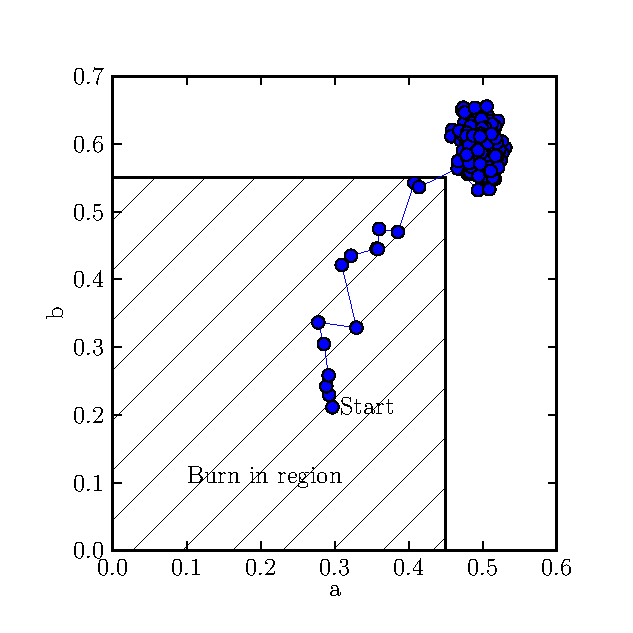
\includegraphics{2d_burn_in}
  \caption{The Markov chain from run \#1 plotted on top of the $\{a,b\}$ parameter space. We can see how the algorithm converged upon a specific of region parameter space. The ``burn in'' region is where the chain was biased by the starting location, and we discard it for all further analysis.}
\label{fig:burn_in}
\end{center}
\end{figure}

\section{Studying your Markov chain}

In every Markov chain, there is usually a period of ``burn in,'' where the jumps in parameter space are biased by the starting location, and do not accurately reflect the overall landscape of the likelihood space. When plotting the chain on top of the $\{a,b\}$ parameter space in Figure~\ref{fig:burn_in}, we can clearly see the burn in region.

\begin{figure}
\begin{center}
  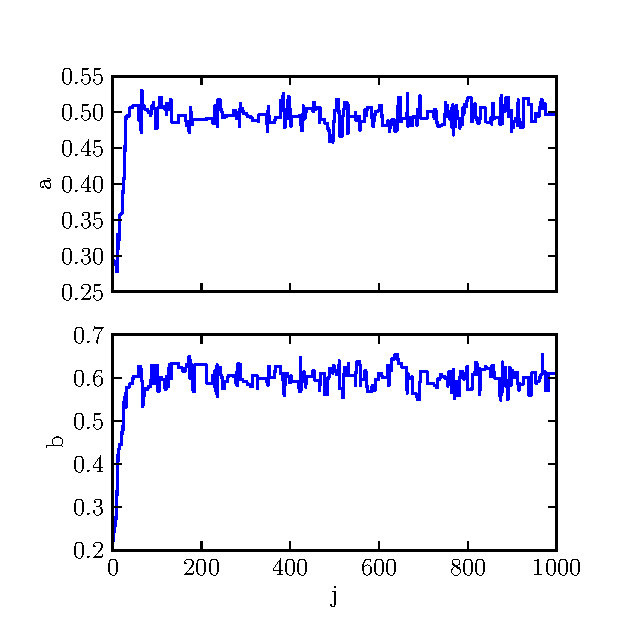
\includegraphics{param_vs_j}
  \caption{Same data plotted in Figure~\ref{fig:burn_in}, but plotted for individual parameters as a function of $j$.}
\label{fig:param_vs_j}
\end{center}
\end{figure}

All subsequent analysis of the chain should be done after discarding the burn-in steps from the Markov chain. All chains referred to in this document can be found with the code as \verb|runX.dat|. The experts say that an acceptance ratio in step \#3 of the Metropolis-Hastings algorithm should be close to 25\%.

In order to determine the best fit parameters of our model (and their errors), we need to examine the Markov chain, since this chain has sampled our likelihood space in a statistically consistent manner. After discarding the burn in region, we bin the values of the chain and plot them in a histogram. This histogram is proportional to the target probability distribution. If we normalize it so that the integral is 1, it is the probability distribution (Figure~\ref{fig:hist_param}). It is from this distribution that we can draw the mean and standard deviation on the parameters. The mean and standard deviation can be determined via standard statistical tasks, for example \verb|Python|'s \verb|np.mean| and \verb|np.std|.

\begin{figure}
\begin{center}
  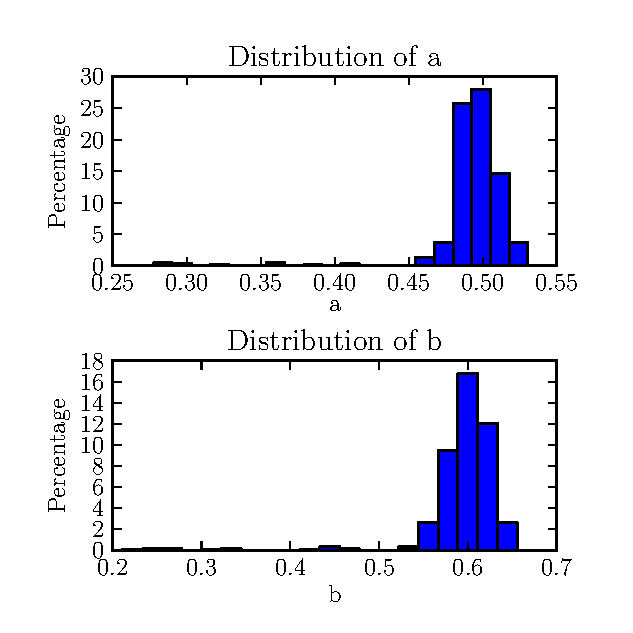
\includegraphics{hist_param}
  \caption{Once normalized to 1, the binned Markov Chain (minus burn in period) is the probability density function of the parameters. The means of these distributions are our best estimates on $a$, $b$ and the widths are our errors $\sigma_a$, $\sigma_b$.}
\label{fig:hist_param}
\end{center}
\end{figure}

\section{Effect of changing step size and starting position}

Now that we have a working MCMC, let's tweak it to see what happens. What is the effect of changing the step size? We run three different chains with different $\Delta\sigma_a$ and $\Delta\sigma_b$, summarized in Table~\ref{table:acceptance}. We see that using jump sizes similar to the original estimates yields the most desirable acceptance ratio. If we choose a step size that is too small, we may have a higher acceptance ratio, but we will also take a longer time to converge upon the most likely parameters. If our likelihood space is not monotonic, and has local maxima, then our chain may have trouble escaping. However, if our step size is too big, then we may oscillate back and forth around the maximum without actually sampling it adequately.

\begin{deluxetable}{lllr}
  \tablecaption{\label{table:acceptance}Step size and acceptance ratio}
  \tablehead{\colhead{Run \#} & \colhead{$\Delta\sigma_a$} & \colhead{$\Delta\sigma_b$} & \colhead{Acceptance (\%)}}
\startdata
1 & 0.03 & 0.05 & 24 \\
2 & 0.01 & 0.02 & 60 \\
3 & 0.05 & 0.10 & 9 \\
\enddata
\tablecomments{For this data set, it appears the ideal step size is close to $\sigma_{a,e}$ and $\sigma_{b,e}$.}
\end{deluxetable}

What is the effect does using different starting parameters have on the parameter estimates? Theoretically, if the algorithm works correctly and we discard our burn-in region properly, then we should obtain similar parameter estimates regardless of our starting position. Table~\ref{table:starting} shows that this is in fact the case. We can see in Figure~\ref{fig:2d_all} that three different chains, each started from a different position, all converge upon the most likely region of parameter space.

\begin{deluxetable}{cccr@{$\pm$}lr@{$\pm$}l}
  \tablecaption{\label{table:starting}Starting position and parameter estimates}
  \tablehead{\colhead{Run \#} & \colhead{$a_{\rm start}$} & \colhead{$b_{\rm start}$} & \multicolumn{2}{c}{$a \pm \sigma_a$} & \multicolumn{2}{c}{$b \pm \sigma_b$}}
\startdata
A & 0.0 & 1.0 & 0.498 & 0.010 & 0.595 & 0.021\\
B & 1.0 & 1.0 & 0.499 & 0.013 & 0.604 & 0.022\\
C & 0.0 & -0.3 & 0.499 & 0.009 & 0.604 & 0.020\\
\enddata
\tablecomments{Each chain done with $\Delta\sigma_a = 0.03$, $\Delta\sigma_b = 0.05$. Runs displayed in Figure~\ref{fig:2d_all}.}
\end{deluxetable}

\begin{figure}
\begin{center}
  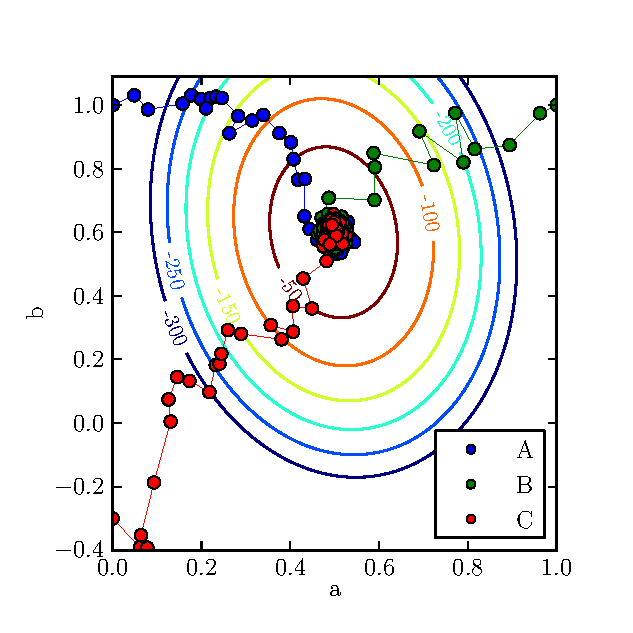
\includegraphics{2d_all}
  \caption{Graphical display of Markov chains in Table~\ref{table:starting}. Note that each chain converges upon the most likely region of parameter space irregardless of starting position.}
\label{fig:2d_all}
\end{center}
\end{figure}

\bibliography{master}
\bibliographystyle{apj}

\end{document}


